\documentclass[11pt]{article}

\usepackage{graphicx}
\usepackage{multirow}
\usepackage{amssymb}
\usepackage{amsmath}
\usepackage[left = 2cm, right = 2cm, top = 2cm, bottom = 2cm]{geometry}
\usepackage{hyperref}
\usepackage{xcolor}
\usepackage{physics}
\usepackage{soul}
\usepackage{subcaption}
\usepackage{verbatim}
\usepackage{listings}

\lstset{basicstyle=\ttfamily,
columns=fullflexible,
frame=single,
breaklines=true,
postbreak=\mbox{\textcolor{red}{$\hookrightarrow$}\space},
language=C++}

\definecolor{red2}{RGB}{255, 49, 49}
\definecolor{green2}{RGB}{144, 238, 144}
\definecolor{purple2}{RGB}{150, 111, 214}
\newcommand{\hlyellow}[1]{{\sethlcolor{yellow}\hl{#1}}}
\newcommand{\hlgreen}[1]{{\sethlcolor{green2}\hl{#1}}}
\newcommand{\hlred}[1]{{\sethlcolor{red2}\hl{#1}}}
\newcommand{\hlpurple}[1]{{\sethlcolor{purple2}\hl{#1}}}

\bibliographystyle{plain}%abbrv} % We choose the "plain" reference style

\title{Notes on Silvaco TCAD Simulations}
% \author{Danush Shekar\\ Supervised by Dr. Zhenyu Ye and Dr. Corrinne Mills}
\date{\today}

\begin{document}

\maketitle
\tableofcontents

\newpage

%\abstract{}%This is my attempt in saving an account of all tips/tricks, notes, and discussions of the simulation tools I have used (mostly related to HEP simulations). In theory, this is also a note to questions and answers I encountered while I studied the subject, and that this notebook should serve as a reference for the doubts my mind stumbles upon in the future.}

\subsection*{Colour legend}
This document will follow a highlighting scheme where text highlighted in different colors mean the following:
\newline
\hlyellow{Yellow coloured text} - Doubts, or sentences that are to be clarified/understood later.\newline
\hlgreen{Green coloured text} - Some takeaways.\newline
%\hlred{Red coloured text} - Mistakes/typos.\newline
\hlpurple{Purple coloured text} - Interesting and unique points, that often are not mentioned explicitly in textbooks/literature.

\section{About}
Silvaco TCAD is one of the major commercial softwares in the current market that offer tools for the simulation of silicon devices. This note in particular will focus on the tools that facilitate the simulation of Silicon sensors utilized in high energy physics experiments. Particular focus will be towards Athena and Atlas. Athena is a "device-technology" simulation tool, and is widely used for simulating the electrical behavior of semiconductor devices. Athena on the other hand, is a "process-technology" simulation tool. It focuses on the simulation of the manufacturing processes involved in creating semiconductor devices, including deposition, etching, diffusion, etc. Both tools are often used hand-in-hand to offer a comprehensive study of the device to be manufactured.

\section{Atlas}
The primary reference used is Silvaco's Atlas User's Manual \cite{silvaco-atlas}. The workflow as given in \cite{silvaco-atlas} is shown below in Figure \ref{fig:atlas-workflow}. In a very primitive sense: we provide inputs to Atlas through Athena output files, and code in DeckBuild. Atlas then provides outputs that can be visualized in TonyPlot. Most of the following subsections will involve working in the DeckBuild level.

\begin{figure}[h]
    \centering
    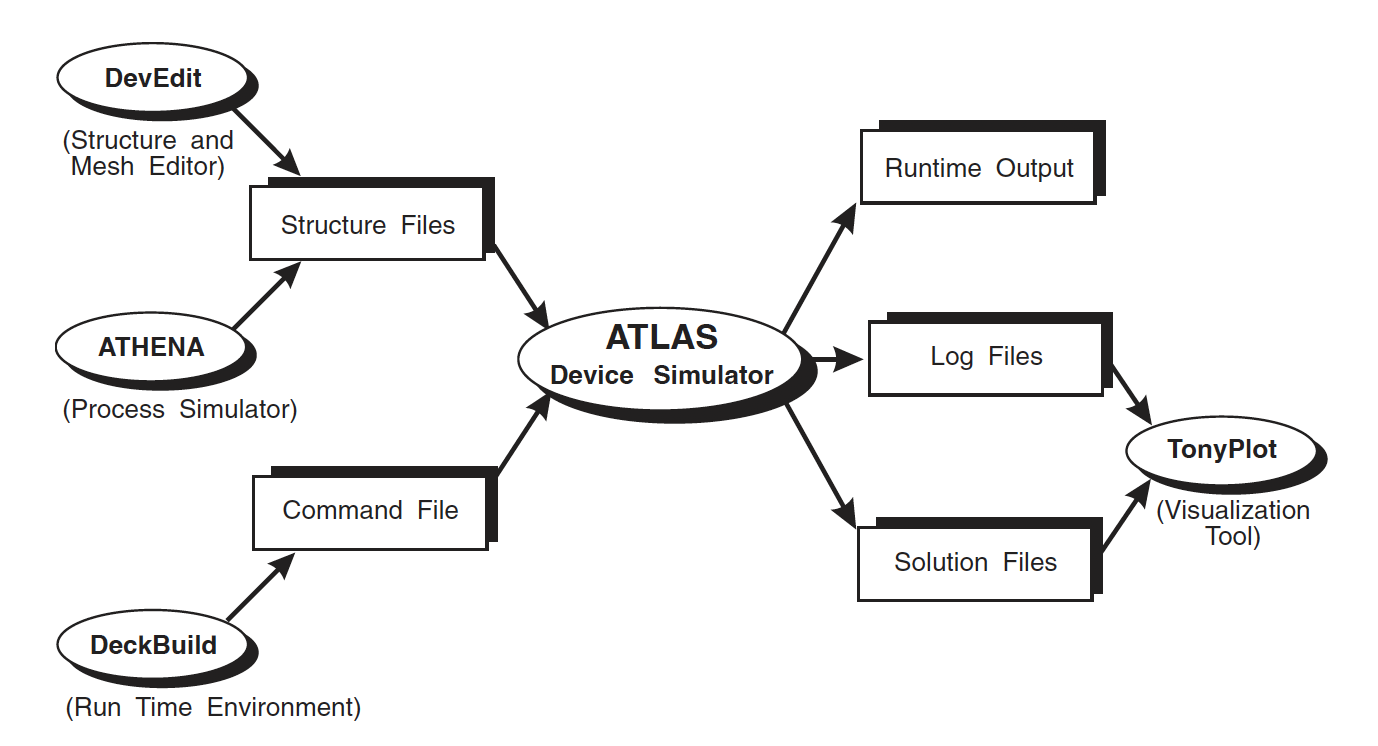
\includegraphics[width=4in]{Images/atlas-input-output.png}
    \caption{.}
    \label{fig:atlas-workflow}
\end{figure}

\subsection{Meshing!}


\bibliography{references}

\end{document}